\documentclass{jsarticle}
\usepackage[dvipdfmx]{graphicx}
\usepackage{listings,jlisting}
\lstset{%
  language={C},
  basicstyle={\small\ttfamily},%
  identifierstyle={\small},%
  commentstyle={\small\itshape},%
  keywordstyle={\small\bfseries},%
  ndkeywordstyle={\small},%
  stringstyle={\small\ttfamily},
  frame={tb},
  breaklines=false,
  columns=[l]{fullflexible},%
  numbers=left,%
  xrightmargin=0zw,%
  xleftmargin=3zw,%
  numberstyle={\scriptsize},%
  stepnumber=1,
  numbersep=1zw,%
  lineskip=-0.5ex%
}

\begin{document}

\title{画像工学 レポート\\ \vspace{1cm}― 画像の2値化 ―\vspace{2cm}}
\author{IE5 (9) 片岡 駿之介 \vspace{1cm}}
\maketitle

\newpage

\section{課題}

画像処理の中に,2値化と呼ばれるものがある.2値化とは,濃淡のある画像を白と黒の2階調に変換する処理のことである.ある閾値を決め,各画素ごとの輝度値が閾値を上回っていれば白,下回っていれば黒に置き換える.この処理を全画素に適用することにより,画像全体で2値化を行うことが出来る.2値化は主に,画像から文字や特定色の領域を抽出すると行った目的で用いられる.\\
本課題では,閾値の計算にモード法と判別分析法(大津の2値化)を用いた2値化処理を実際に実装し,結果を確認する.

\section{処理の流れ}

今回の演習では,PGMファイルを以下の手順で処理していくこととした.
\begin{enumerate}
  \item 入力されたコマンドが正しいかチェック(正しくない場合はUsageを表示して終了)
  \item コマンドで指定されたPGMファイルを読み込む
  \item 読み込んだPGMファイルのヘッダ解析
  \item ヘッダが正しければ画素値を2次元配列に取り込む
  \item コマンドで指定された方法で閾値の計算を行う
  \item 計算した閾値を元に2値化処理を行う
  \item コマンドで指定されたファイルへ画像を出力する
\end{enumerate}

この処理によって得られたPGMファイルをImageMagickを用いて表示し,2値化の結果を比較検討する.\\
\newpage

\section{ソースリスト}

\begin{lstlisting}[caption=binarization.c,label=ほげ]
#include <stdio.h>
#include <stdlib.h>
#include <string.h>
#include <ctype.h>

FILE *fp;

int width;
int height;
int max_value;
int status;
char buffer[128];

void image_open(char *file_name) {
  if ((fp = fopen(file_name, "r")) == NULL) {
		printf("file open error!!\n");
		exit(-1);	/* (3)エラーの場合は通常、異常終了する */
	}
}

int main(int argc,char *argv[]) {

  /* 入力コマンドのチェック */
  if(argc != 4) {
    printf("Usage : ./binarization <binarization type> <input pgm filename> <output pgm filename>\n");
    exit(0);
  } else if (argc == 4) {
    image_open(argv[2]);
    printf("mode : %s\n", argv[1]);
  }

  /* ヘッダ取得部 */
  int ch;

  while (status < 3) {
    ch = getc(fp);

    if(ch == '#') { // コメントのスキップ
      while (( ch = getc(fp)) != '\n')
        break;
    }

    if(ch == 'P') { // マジックナンバーのチェック
      if(getc(fp) != '5') {
        printf("Magic Number is wrong.\n");
        break;
      } else {
        // printf("Magic Number is P5\n");
      }
    }

    if(isdigit((unsigned char)ch)) { // 数値取得部
      buffer[0] = ch;
      int i=1;
      while(1) {
          char c = getc(fp);
          if(isdigit((unsigned char)c)) {
            buffer[i]=c;
            i++;
          } else
            break;
      }
      buffer[i] = '\0';

      switch (status) {
        case 0: // width取得部
          width = atoi(buffer);
          printf("width=%d\n", width);
          break;
        case 1: // height取得部
          height = atoi(buffer);
          printf("height=%d\n", height);
          break;
        case 2: // max_value取得部
          max_value = atoi(buffer);
          printf("max_value=%d\n", max_value);
          break;
      }
      status++; // 次のステータスへ
    }
  }

  /* 画素値取得部 */
  int image[width][height];

  for(int i = 0; i < height; i++) {
    for(int j = 0; j < width; j++) {
      image[j][i] = (int)getc(fp);
    }
  }

  /* ヒストグラム生成部 */
  int histogram[max_value];
  for(int i=0; i <= max_value; i++)
    histogram[i] = 0; //ヒストグラム用配列の初期化

  for(int i=0; i < width; i++) {
    for(int j=0; j < height; j++) {
      histogram[image[j][i]]++;
    }
  }

  /* 閾値計算部 */

  int threshold = 0;

  int output_image[width][height];

  for(int i=0; i < height; i++) {
    for(int j=0; j < width; j++) {
      output_image[j][i] = image[j][i];
    }
  }

  if(strcmp(argv[1], "mode") == 0) { //モード法

    int dHist[max_value-1]; //微分ヒストグラム用の配列
    for(int i=0; i <= (max_value-1); i++) {
      dHist[i] = histogram[i] - histogram[i+1]; //微分ヒストグラム用配列の計算
      // printf("i=%d, dHist[i]=%d \n", i, dHist[i]);
    }

    int range = 40; //最頻値検出用の微分ヒストグラムの探索幅
    int valley = 0; //谷の画素値
    int valley_first = 1;

    for(int i = range; i < (max_value - range); i++) {
      int minus_range = 0;
      int plus_range = 0;

      for(int j = 0; j <= range; j++) { //両側レンジの微分ヒストグラムの合計値の計算
        minus_range = minus_range + dHist[i-j];
        plus_range = plus_range + dHist[i+j];
      }

      printf("i = %d, minus_range = %d, plus_range = %d\n", i, minus_range, plus_range);

      if(minus_range >= 0 && plus_range <= 0) { //マイナス側レンジが右下がりの傾き かつ プラス側レンジが右上がりの傾きのとき
        if(valley_first == 1 || histogram[valley] > histogram[i]) //現在のヒストグラムの値がvalleyより低ければvalleyを更新
          valley = i;
          if(valley_first == 1)
            valley_first = 0;
      }
    }

    printf("valley=%d\n", valley);

    threshold = valley;

    for(int k=0; k <= max_value; k++) {
      // printf("%4d %5d\n", k, histogram[k]);
    }

  } else if(strcmp(argv[1], "otsu") == 0) { //判別分析法(大津の2値化)

    int min = -1; //最小値
    int max = -1; //最大値
    int sum = 0;

    for(int i = 0; i <= max_value; i++) { //平均値、最小値、最大値を求める
      sum += (histogram[i] * i);

      if(histogram[i] != 0) { //その輝度値に画素が存在している場合
        if(min == -1)
          min = i;

        max = i;
      }
    }

    if(min == -1 || max == -1)
      exit(-1);

    float ave = sum / (width * height);
    printf("Average : %f, Max : %d, Min : %d\n", ave, max, min);

    /* 分離度Sを求め、閾値を決める */
    int s = 0; //分離度S

    for(int t = min; t < max; t++) {
      int n1 = 0; //tより左側の画素数の合計
      int v1 = 0; //tより左側の画素値の合計
      int n2 = 0; //tより右側の画素数の合計
      int v2 = 0; //tより右側の画素値の合計

      for(int j = min; j <= max; j++) {
        if(j <= t) {
          n1 += histogram[j];
          v1 += (histogram[j] * j);
          // printf("j : %d, n1 : %d, v1 : %d\n", j, n1, v1);
        } else {
          n2 += histogram[j];
          v2 += (histogram[j] * j);
          // printf("j : %d, n2 : %d, v2 : %d\n", j, n2, v2);
        }
      }

      float ave1 = (float)(v1 / n1); //tより左側の画素値の平均
      float ave2 = (float)(v2 / n2); //tより右側の画素値の平均

      float sum1 = 0; //tより左側の平均との差の二乗を足し込む変数
      float sum2 = 0; //tより右側の平均との差の二乗を足し込む変数

      for(int j = min; j <= max; j++) {
        if(j <= t)
          sum1 += ((j - ave1) * (j - ave1));
        else
          sum2 += ((j - ave2) * (j - ave2));
      }

      float sigma_1 = sum1 / n1; //tより左側の分散
      float sigma_2 = sum2 / n2; //tより右側の分散

      float sigma_w = (n1 * sigma_1 + n2 * sigma_2) / (n1 + n2); //クラス内分散
      float sigma_b = (n1 * ((ave1 - ave) * (ave1 - ave)) + n2 * ((ave2 - ave) * (ave2 - ave))) / (n1 + n2); //クラス間分散

      int s_local = sigma_b / sigma_w; //分離度の計算

      if(s_local > s) {//分離度が大きければ閾値を更新
        s = s_local;
        threshold = t;
      }
    }
  }

  printf("threshold : %d\n", threshold);
  /* 2値化処理 */

  for(int i = 0; i < height; i++) {
    for(int j = 0; j < width; j++) {
      if(image[j][i] > threshold)
        output_image[j][i] = max_value;
      else
        output_image[j][i] = 0;
    }
  }

  /* 画像出力部 */

  FILE *output = fopen(argv[3], "wb");
  char header[30];
  sprintf(header, "P5 %d %d %d\n", width, height, max_value);
  fputs(header, output);
  for(int i = 0; i < height; i++) {
    for(int j = 0; j < width; j++) {
      fputc((char)output_image[j][i], output);
    }
  }
  printf("image was output.\n");
  fclose(output);
}


\end{lstlisting}

\newpage

\section{実験}
検証用画像として,「cameraman.pgm」「source.pgm」「town.pgm」を用意した.\\
それぞれの検証用画像を以下に示す.

\begin{figure}[htbp]
 \begin{minipage}{0.33\hsize}
  \begin{center}
   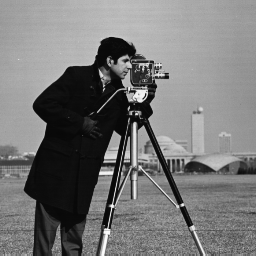
\includegraphics[height=40mm]{cameraman.png}
  \end{center}
  \caption{cameraman.pgm}
  \label{fig:one}
 \end{minipage}
 \begin{minipage}{0.33\hsize}
  \begin{center}
   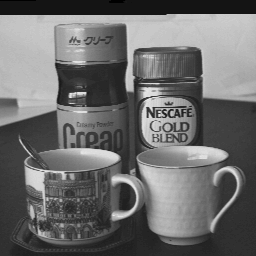
\includegraphics[height=40mm]{source.png}
  \end{center}
  \caption{source.pgm}
  \label{fig:two}
 \end{minipage}
 \begin{minipage}{0.33\hsize}
  \begin{center}
   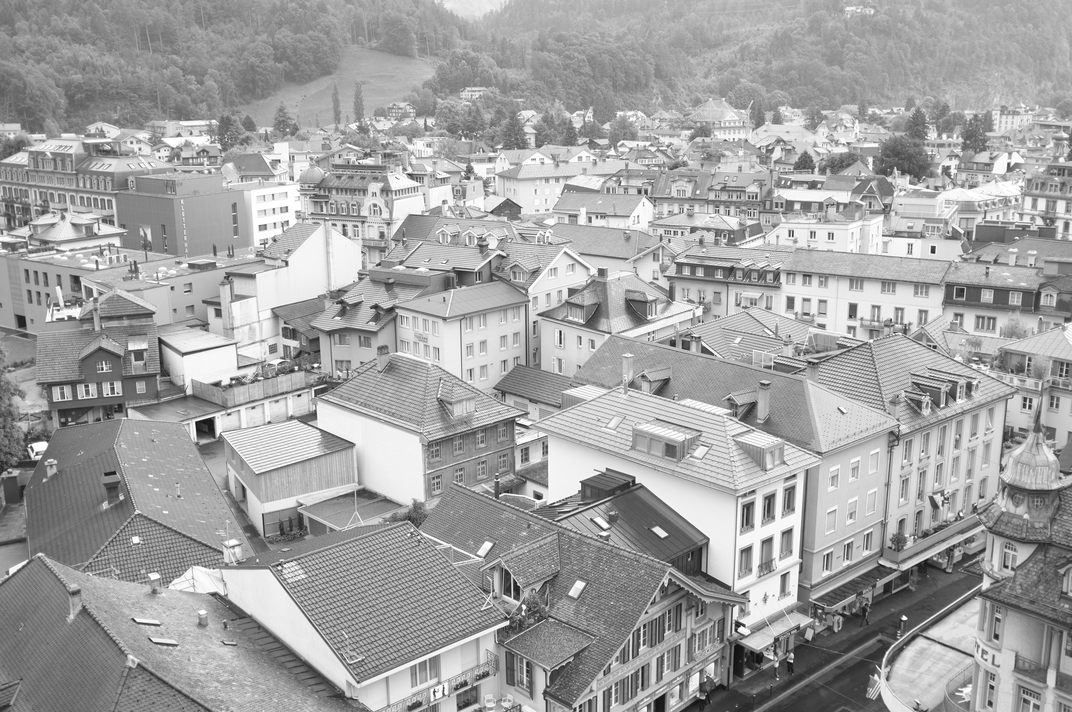
\includegraphics[height=40mm]{town.png}
  \end{center}
  \caption{town.pgm}
  \label{fig:three}
 \end{minipage}
\end{figure}

また,これらの検証用画像のヒストグラムを以下に示す.
\begin{figure}[htbp]
 \begin{minipage}{0.33\hsize}
  \begin{center}
   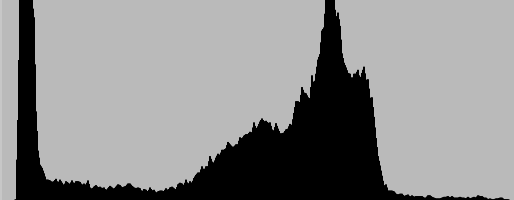
\includegraphics[height=20mm]{cameraman_histogram.png}
  \end{center}
  \caption{cameraman.pgm}
  \label{fig:one}
 \end{minipage}
 \begin{minipage}{0.33\hsize}
  \begin{center}
   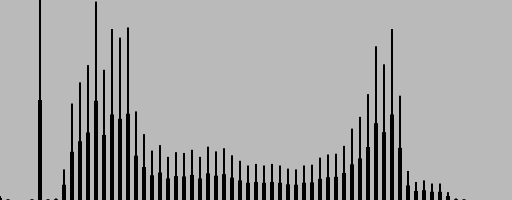
\includegraphics[height=20mm]{source_histogram.png}
  \end{center}
  \caption{source.pgm}
  \label{fig:two}
 \end{minipage}
 \begin{minipage}{0.33\hsize}
  \begin{center}
   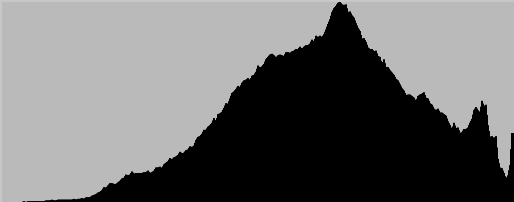
\includegraphics[height=20mm]{town_histogram.png}
  \end{center}
  \caption{town.pgm}
  \label{fig:three}
 \end{minipage}
\end{figure}


\subsection{モード法}
モード法により閾値を決定する際には,双峰型ヒストグラムの谷を検出することが重要である.今回,谷の検出には以下の手法を用いた.
\begin{enumerate}
  \item 画像のヒストグラムを微分していき,傾きをdHist配列に格納する
  \item 1の処理を0〜max\_valueで繰り返し行う
  \item 対象とする輝度値から左右range変数分の合計値を求め,minus\_range変数とplus\_range変数にそれぞれ代入する
  \item もしマイナス側レンジが0以上かつプラス側レンジが0以下だった場合(すなわち,極小値を取る場合),谷の輝度値を更新する
  \item 3と4の処理を繰り返し行い,最後に谷の輝度値を閾値として設定する
\end{enumerate}
この方法を用いて,検証用画像に対して2値化処理を行った結果を以下に示す.
\begin{figure}[htbp]
 \begin{minipage}{0.33\hsize}
  \begin{center}
   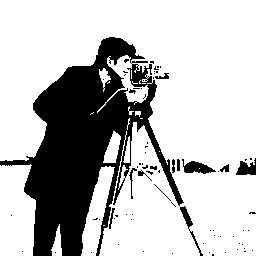
\includegraphics[height=40mm]{mode-cameraman.png}
  \end{center}
  \caption{cameraman.pgm}
  \label{fig:one}
 \end{minipage}
 \begin{minipage}{0.33\hsize}
  \begin{center}
   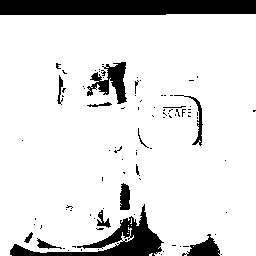
\includegraphics[height=40mm]{mode-source.png}
  \end{center}
  \caption{source.pgm}
  \label{fig:two}
 \end{minipage}
 \begin{minipage}{0.33\hsize}
  \begin{center}
   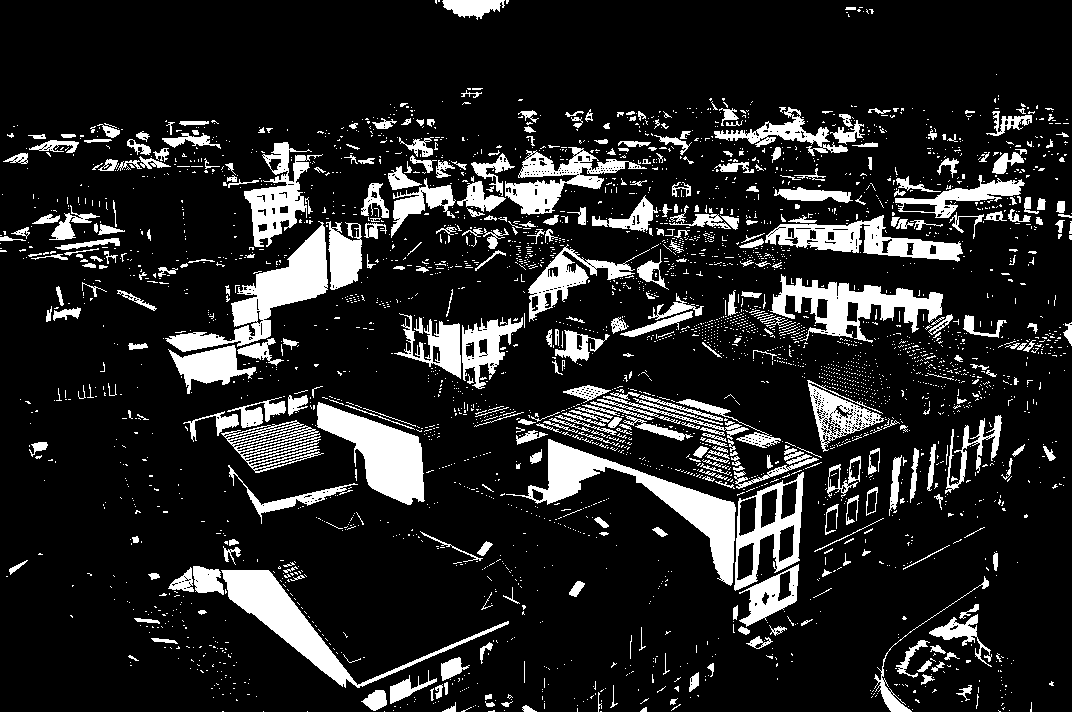
\includegraphics[height=40mm]{mode-town.png}
  \end{center}
  \caption{town.pgm}
  \label{fig:three}
 \end{minipage}
\end{figure}

\subsection{判別分析法(大津の2値化)}
判別分析法は,クラス間分散とクラス内分散の比で求められる分離度を求め,この分離度が最大となるときの輝度値を閾値とするものである.
今回,判別分析法を以下の方法に寄って実装した.
\begin{enumerate}
  \item 画像全体の平均値,最小値,最大値を求める
  \item 分離度を求める
  \item もし分離度が現在の分離度よりも大きければ,分離度を更新し,そのときの輝度値を記録
  \item 2と3の処理を0〜max\_valueで繰り返し行う
  \item 分離度が最大のときの輝度値を閾値とする
\end{enumerate}
この方法を用いて,検証用画像に対して2値化処理を行った結果を以下に示す.
\begin{figure}[htbp]
 \begin{minipage}{0.33\hsize}
  \begin{center}
   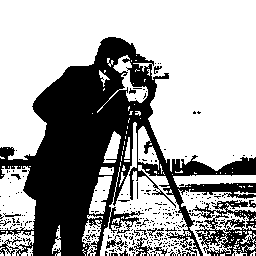
\includegraphics[height=40mm]{otsu-cameraman.png}
  \end{center}
  \caption{cameraman.pgm}
  \label{fig:one}
 \end{minipage}
 \begin{minipage}{0.33\hsize}
  \begin{center}
   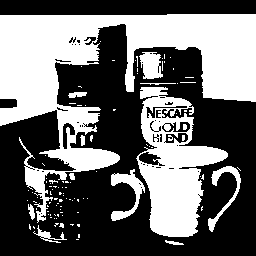
\includegraphics[height=40mm]{otsu-source.png}
  \end{center}
  \caption{source.pgm}
  \label{fig:two}
 \end{minipage}
 \begin{minipage}{0.33\hsize}
  \begin{center}
   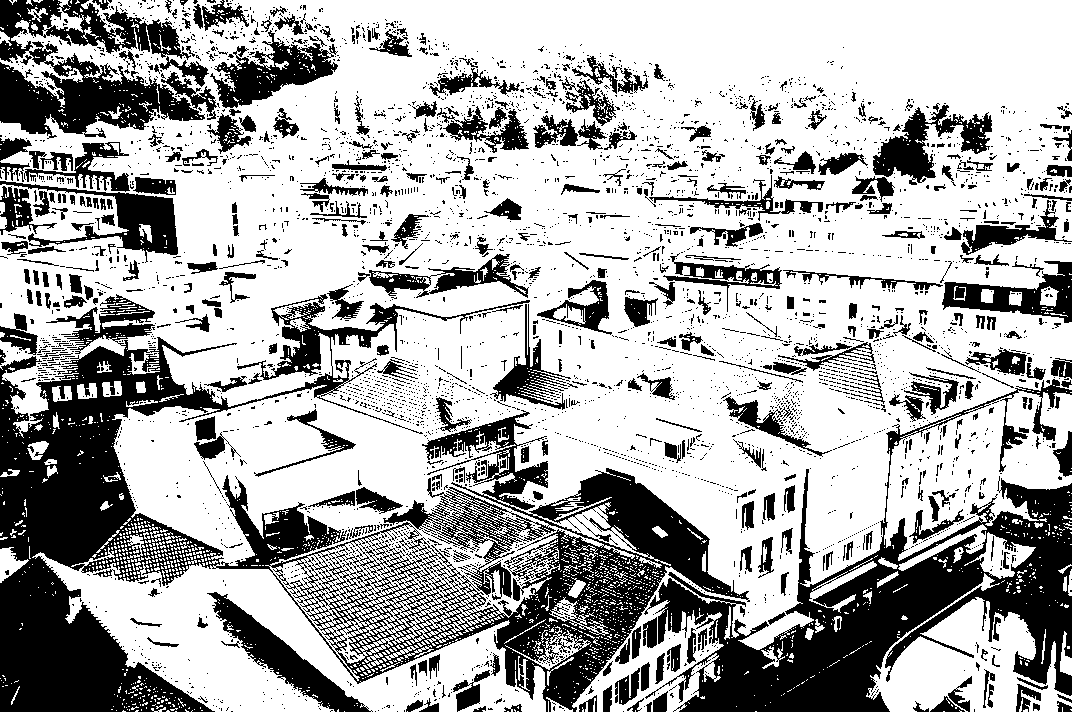
\includegraphics[height=40mm]{otsu-town.png}
  \end{center}
  \caption{town.pgm}
  \label{fig:three}
 \end{minipage}
\end{figure}


\section{考察}
\subsection{モード法}
連続的な双峰型ヒストグラムとなっている「cameraman.pgm」では,理想的な2値化が行われているように感じられる.\\
「source.pgm」は双峰型ヒストグラムであるが,輝度値が離散的なため,今回の実装手法では谷の探索が正確に行えず,理想的な2値化とは言い難い結果となった.\\
「town.pgm」はそもそも双峰型ヒストグラムではないため,モード法では理想的な2値化が行われていない.\\

「cameraman.pgm」のような,なだらかな双峰型ヒストグラムでは良好な結果が得られるが,他の2枚のような状況では良好な結果が得られず,使い所がかなり限られてしまうことがわかった.

\subsection{判別分析法(大津の2値化)}
大津の2値化では,3枚ともかなり良好な結果が得られた.
こちらはモード法に比べて,どのようなヒストグラムでも安定的に2値化を行うことが出来るため,非情に使い易いアルゴリズムであることがわかった.

\section{感想}
今回は2値化処理の実装を行ったが,モード法では自分でアルゴリズムを考案し,今まで自分の中ではあやふやだった画像の微分処理の本質を理解することができたので良かった.ただ,このモード法の実装方法は必ずしも良いモノとは言えないので,さらに突き詰める必要が有るようにも感じる.\\
また,大津の2値化は工学セミナーなどでアルゴリズム自体は聞いたことがあったが,実際に自分で実装したことはなかったので良い経験になった.

\end{document}
